\begin{frame}
\frametitle{Hardware used in this training session}
  Using Microchip (formerly Atmel) SAMA5D3 Xplained boards in all practical labs
  \begin{columns}
    \column{0.6\textwidth}
    {\footnotesize
    \begin{itemize}
	\item SAMA5D36 (Cortex A5) CPU from Microchip
	\item USB powered!
	\item 256 MB DDR2 RAM, 256 MB NAND flash
	\item 2 Ethernet ports (Gigabit + 100 Mbit)
	\item 2 USB 2.0 host, 1 USB device
	\item 1 MMC/SD slot
	\item 3.3 V serial port (like Beaglebone Black)
	\item Misc: Arduino R3-compatible header, JTAG, buttons, LEDs
	\item Currently sold at 102 EUR by Mouser (V.A.T. not included)
    \end{itemize}
    }
    \column{0.4\textwidth}
    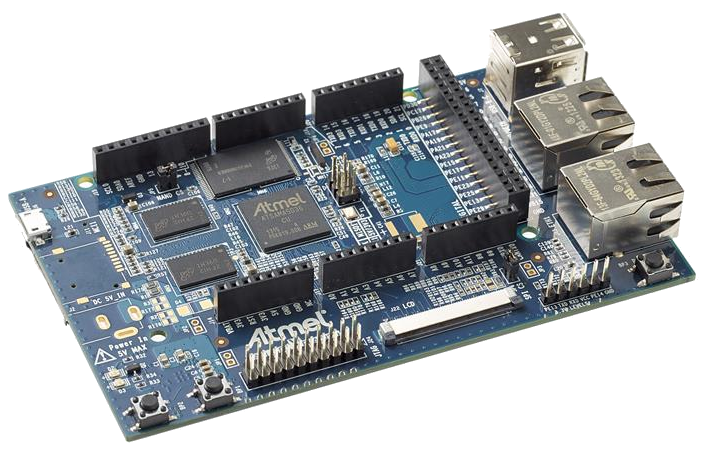
\includegraphics[width=\textwidth]{slides/xplained-board/xplained-board.png}
  \end{columns}
  \vspace{1em}
  {\small
  Board and CPU documentation, design files, software:
  \url{https://bit.ly/2Ghv10p} (Microchip's website)
  }
\end{frame}
